\chapter{The Standard Model and Its Future}\label{sec:theory}

In Section \ref{sec:introduction}, we introduced the few obstacles facing the SM: Existance of darkmatter, baryon-antibaryon asymmetry, and the evidence of neutrino masses and mixing. 
The SM Lagrangian, writted as in formula \ref{eq:SM}, does not have particles' fields to explain these phenomena.
\begin{equation}
\label{eq:SM}
\mathcal{L}_{SM} = \mathcal{L}_{Higgs}+\mathcal{L}_{Gauge}+\mathcal{L}_{Kinetic}+\mathcal{L}_{Yukawa}
\end{equation}
\begin{align*}
\end{align*}
Since it can not be explained by any of the particles' fields in the SM, it requires addition of new particles' fields or new terms in the current SM Lagrangian expression.
New terms in the SM Lagrangian entails in new vertices in the Feynman diagram, which open the door for a new understanding of the high energy physics.
However, if those observations did not exist, the SM is all complete within its own framework, only except for the naturalness problem.

The naturalness problem originates from the fact that the SM Higgs is a scalar particle.
The formula \ref{eq:SM} has three different kinds of fields: boson, fermion, and scalar.
Quantum Field Theory (QFT), the humanity's  mathematical framework used for the SM, explains matter as an excited state of fermion fields, derived from the canonical quantization of the SM Lagrangian's fermion fields.
The fermions' fields have chrial symmetry as demostrated in the kinetic term of the SM Lagrangian in formula \ref{eq:Lag1}.
\begin{equation}
\label{eq:Lag1}
	\mathcal{L}_{Yukawa}  = -Y_{f}\bar{f}_{L}^{i}\Phi_{i}f_{R} +h.c.
	\mathcal{L}_{Kinetic} = -Y_{f}\bar{f}_{L}^{i}\Phi_{i}f_{R} +h.c.
\end{equation}
\begin{align*}
\end{align*}
%	\caption{The QFT explains forces of the universe as exchange of boson particles among the fermions, which can be derived from the fermion kinetic term of the SM Lagrangian.}
Likewise, the bosons' fields also satify special symmetries in the QFT framework.
The boson satisfy the U(1), SU(2) or SU(3) gauge symmetry, and are expressed in gauge terms as in formula \ref{eq:Lag2}.
\begin{equation}
\label{eq:Lag2}
	\mathcal{L}_{Gauge} = -Y_{f}\bar{f}_{L}^{i}\Phi_{i}f_{R} +h.c.
\end{equation}
\begin{align*}
\end{align*}
%	\caption{The QFT explains forces of the universe as exchange of boson particles among the fermions, which can be derived from the fermion kinetic term of the SM Lagrangian.}
QFT Renormalization
These chrial and gauge symmetries protect fermion and boson fields from the radiative correction in the renormalization process.

Unlike fermions or gauge bosons, its mass is not protected by any symmetry and is subject to large radiative corrections, especially from the top quark loop. 
Thus, for the SM to be valid up to the Planck or Grand Unification Theory (GUT) scales, the necessary radiative corrections are enormous. 
One needs an exorbitant amount of fine-tuning to fit the Higgs mass at the observed value of 125GeV.
One of the most popular solutions to this problem is Supersymmetry (SUSY), which assigns chirality to the Higgs particle. 
SUSY solves the fine-tuning problem, neutrino masses, and provides a candidate for DM. 
Unfortunately, the LHC has found no significant excess over the SM background in their search for SUSY\cite{SUSY}. 
Although the non-observation of supersymmetric partner particles does not invalidate SUSY, it makes less attractive among the particle physics community. 
Non-observation of superpartners, particularly the stop (scalar partner of the top quark) has pushed its mass beyond 1TeV. 
This generates "little hierarchy" problem, but an alternative solution of "neutral naturalness" remains. 

In the framework of neutral naturalness, the top partners are not charged under the SM color group. 
Because of being colorless, their production crosssection is much smaller, and the present limits on the top partner particles are well below 1TeV. 
Examples of neutral naturalness models are the Twin Higgs \cite{Chacko:2005pe},
Folded SUSY \cite{Burdman:2006tz}, and the Quirky Little Higgs \cite{Cai:2008au} models.
Theoretical models provide the possibility of neutral Long-Lived Particles (LLPs), which may be produced in the proton-proton
collisions of the LHC, and decay back to SM particles far from the interaction point (IP).\cite{Craig:2015pha}
If the mirror QCD gluons form scalar glueballs, the SM Higgs boson can become a "Higgs Portal" between the SM and BSM mirror QCD scalar glueballs. 
In the Mirror SM and Twin SM models, only the SM Higgs boson can interact with both SM QCD and mirror QCD particles.
BSM mirror QCD scalar glueballs can only decay back to SM particles via Higgs boson decay as well. 
Because of its decay as an offshell Higgs boson, its crosssection is highly suppressed. 
Decay branching ratio to highest mass fermions will be highest following the Yukawa couplings.
Decay ratio into b quarks or tau leptons are highest depending on the mirror scalar's mass.
The displaced decays of the scalars would lead to exotic signatures in the CMS, such as distant innermost tracker hit, displaced vertices, and displaced jets.
Phenomenology of long-lived particles in LHC entailed increase in interest of neutral naturalness framework among the particle physics community. \cite{Curtin:2015fna,Csaki:2015fba}.
The long-lived scalar model is shown in the Figure (to be made soon).

\begin{figure}[h!]
  \caption{A cartoon display of Higgs Portal process}
  \label{fig:HiggsPortal}
  \centering
  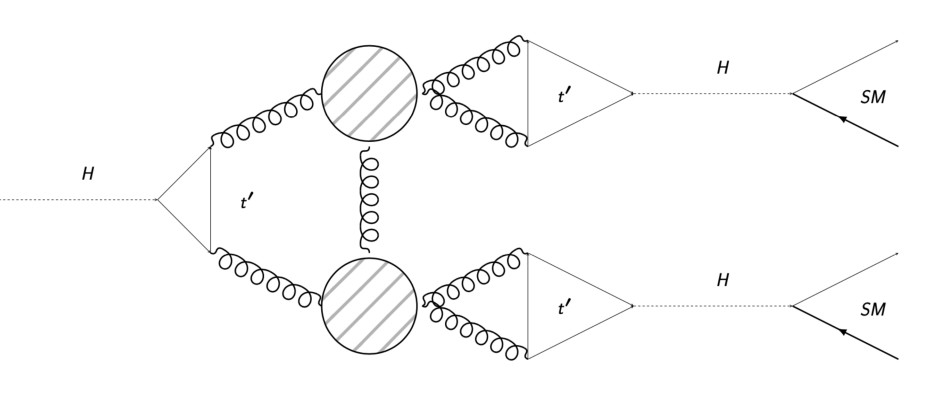
\includegraphics[width=0.87\linewidth]{figs/TwinHiggs.png}
\end{figure}
\begin{figure}[h!]
  \caption{A cartoon display of Higgs Portal process}
  \label{fig:2HiggsPortal}
  \centering
  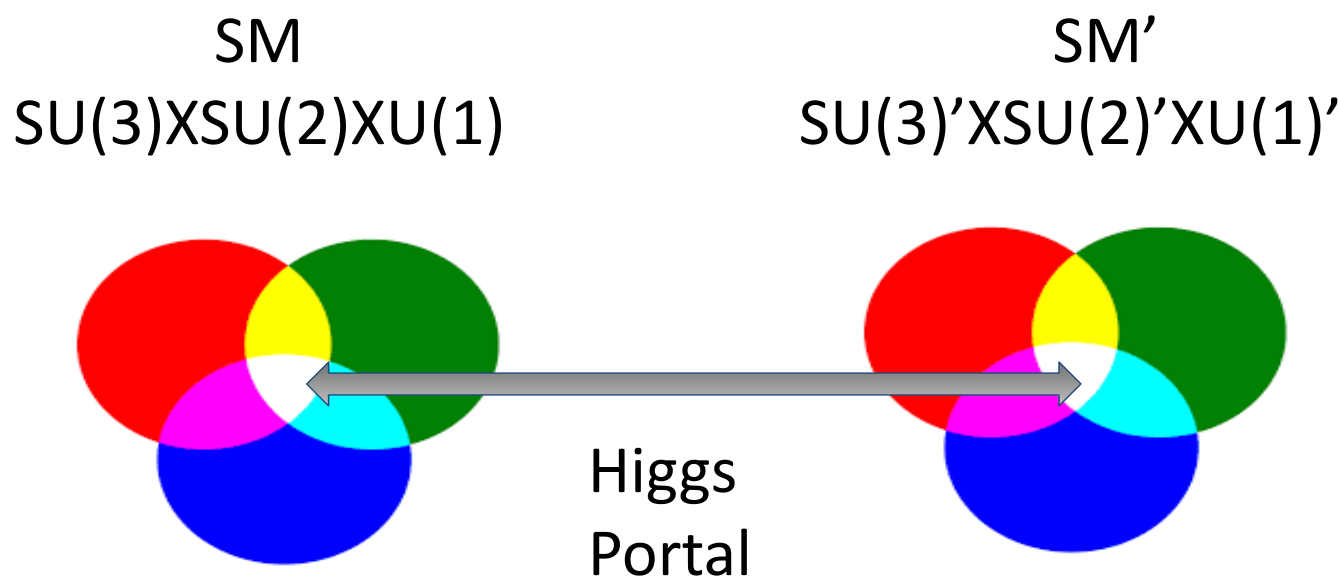
\includegraphics[width=0.87\linewidth]{figs/Portalcartoon.png}
\end{figure}
